\subsection{Bifurcação}

%--------------------

\begin{frame}
\vspace{5pt}
\frametitle{Família Quadrática: \subsecname}
\begin{columns}
\column{\dimexpr\paperwidth-15pt}

\begin{definition}
Seja $f_\lambda$ uma família parametrizada de funções no parâmetro $\lambda$. Dizemos que a família sofre uma bifurcação em $\lambda_0$ se existe $\varepsilon > 0$ com a seguinte propriedade: se $\lambda_1 \in (\lambda_0 - \varepsilon, \lambda_0)$ e $\lambda_2 \in (\lambda_0, \lambda_0 + \varepsilon)$, então $f_{\lambda_1}$ e $f_{\lambda_2}$ não são topologicamente conjugadas.
\end{definition}

\end{columns}
\end{frame}

%--------------------

\begin{frame}
\vspace{5pt}
\frametitle{Família Quadrática: \subsecname}
\begin{columns}
\column{\dimexpr\paperwidth-15pt}

\begin{block}{Exemplo}
A família $E_\lambda$ de funções dadas por $E_\lambda(x) = e^{x + \lambda}$ sofre uma bifurcação em $\lambda_0 = -1$.

\vspace{10pt}

\begin{figure}[!htb]
\centering
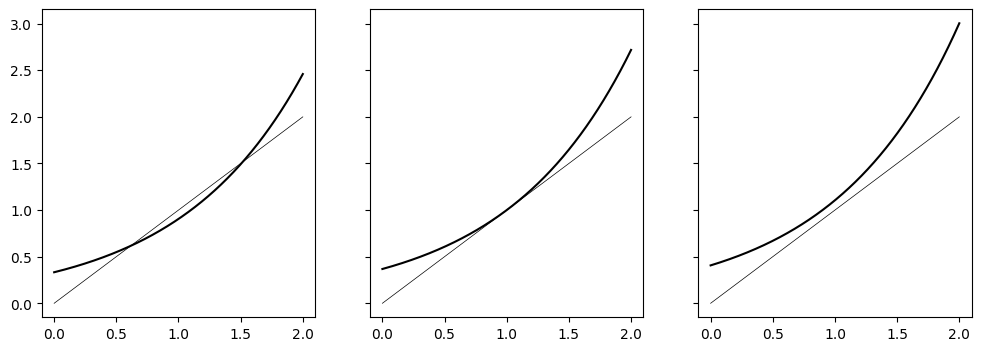
\includegraphics[scale=0.4]{images/e_lambda.png}
\caption{Gráficos de $E_\lambda$ numa vizinhança de $1$ para $\lambda = -1.1$, $\lambda = -1$ e $\lambda = -0.9$.}
\end{figure}
Uma bifurcação com essas características é chamada de bifurcação tangente.
\end{block}

\end{columns}
\end{frame}

%--------------------

\begin{frame}
\vspace{5pt}
\frametitle{Família Quadrática: \subsecname}
\begin{columns}
\column{\dimexpr\paperwidth-15pt}

\begin{block}{Exemplo}
A família quadrática sofre uma bifurcação em $\mu_0 = 3$.

\vspace{10pt}

\begin{figure}[!htb]
\centering
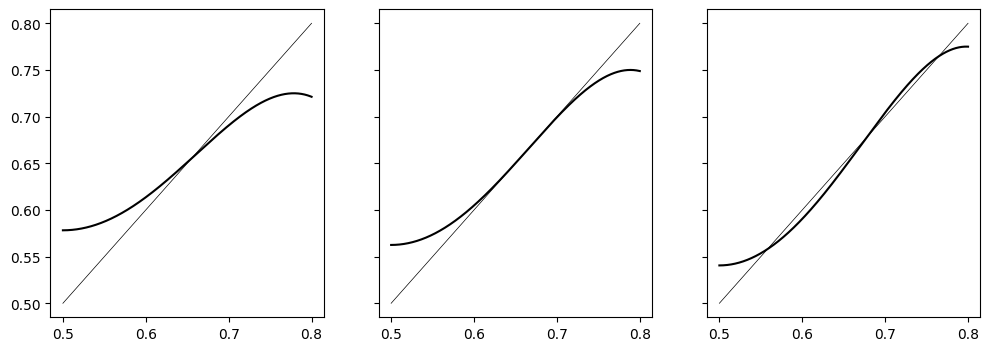
\includegraphics[scale=0.4]{images/h_3^2.png}
\caption{Gráficos de $h^2$ numa vizinhança de $p_\mu$ para $\mu = 2.9$, $\mu = 3$ e $\mu = 3.1$.}
\end{figure}
Uma bifurcação com essas características é chamada de bifurcação com duplicação de período.
\end{block}

\end{columns}
\end{frame}

%--------------------

\begin{frame}
\vspace{5pt}
\frametitle{Família Quadrática: \subsecname}
\begin{columns}
\column{\dimexpr\paperwidth-15pt}

Vamos estudar com mais detalhes a bifurcação com duplicação de período que ocorre na família quadrática.

Se $\mu > 2$, então existe $p_\mu' < p_\mu$ tal que $h(p_\mu') = p_\mu$.
Na figura abaixo temos, para alguns valores de $\mu$, gráficos de $h^2$ juntamente com quadrados limitados por $p_\mu'$ e $p_\mu$.

\begin{figure}[!htb]
\centering
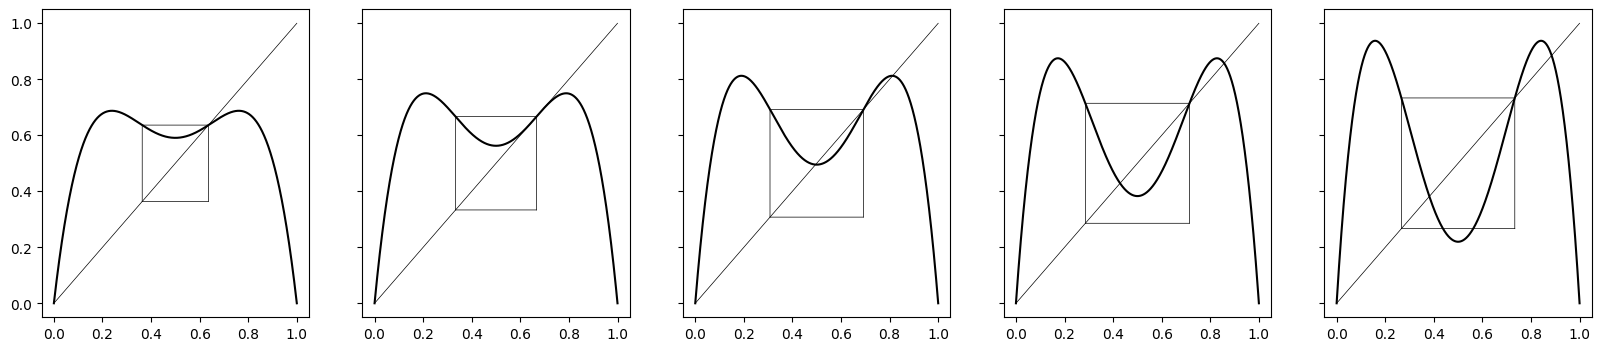
\includegraphics[scale=0.375]{images/h^2withboxes.png}
\caption{Gráficos de $h^2$ para $\mu = 2.75$, $\mu = 3$, $\mu = 3.25$, $\mu = 3.5$ e $\mu = 3.75$.}
\label{h^2-and-boxes}
\end{figure}

\end{columns}
\end{frame}

%--------------------

\begin{frame}
\vspace{5pt}
\frametitle{Família Quadrática: \subsecname}
\begin{columns}
\column{\dimexpr\paperwidth-15pt}

Se $L: [p_\mu', p_\mu] \to [0, 1]$ é a função linear tal que $L(p_\mu') = 1$ e $L(p_\mu) = 0$, então definimos a renormalização de $h$ como a função $Rh: [0, 1] \to [0, 1]$ dada por
$$Rh(x) = L \circ h^2 \circ L^{-1}(x).$$

\begin{figure}[!htb]
\centering
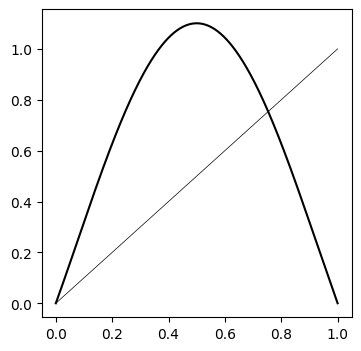
\includegraphics[scale=0.4]{images/renormalization.png}
\caption{Gráfico de $Rh$ para $\mu = 3.75$.}
\label{renormalization}
\end{figure}

\end{columns}
\end{frame}

%--------------------

\begin{frame}
\vspace{5pt}
\frametitle{Família Quadrática: \subsecname}
\begin{columns}
\column{\dimexpr\paperwidth-15pt}

Observando a semelhança de $Rh$ com $h$, esperamos que $Rh$ sofra uma bifurcação com duplicação de período conforme o parâmetro cresce e, desse modo, podemos fazer repetir a análise feita anteriormente. Continuando esse processo, criamos uma sucessão de bifurcações com duplicação de período na família quadrática.

\end{columns}
\end{frame}

%--------------------

\begin{frame}
\vspace{5pt}
\frametitle{Família Quadrática: \subsecname}
\begin{columns}
\column{\dimexpr\paperwidth-15pt}

Com auxílio de um computador, podemos observar as bifurcações com duplicação de período que ocorrem na família quadrática.

\begin{figure}[!htb]
\centering
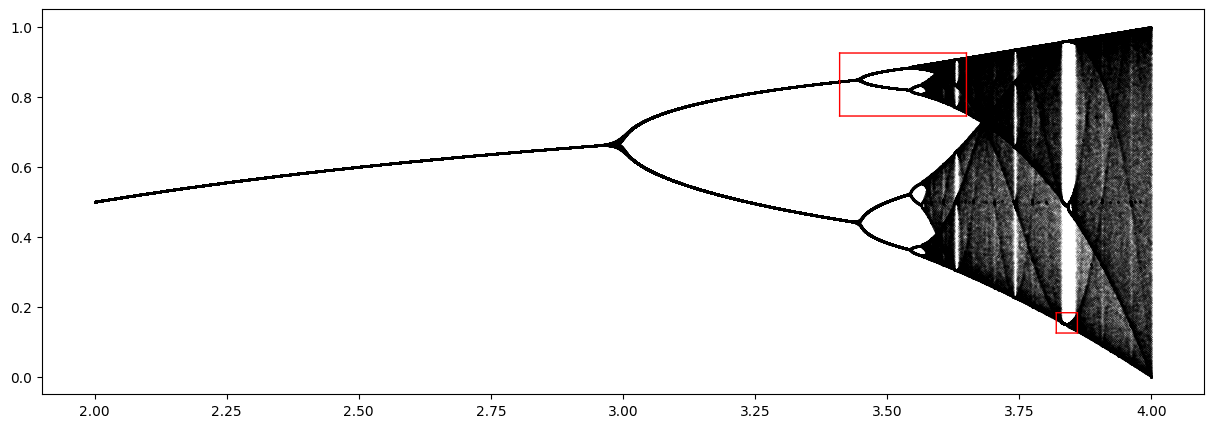
\includegraphics[scale=0.4]{images/period-doubling-and-zoom1.png}
\caption{Diagrama de órbita de $h$ para $2 \leq \mu \leq 4$.}
\end{figure}

\end{columns}
\end{frame}

%--------------------

\begin{frame}
\vspace{5pt}
\frametitle{Família Quadrática: \subsecname}
\begin{columns}
\column{\dimexpr\paperwidth-15pt}

\begin{figure}[H]
\centering
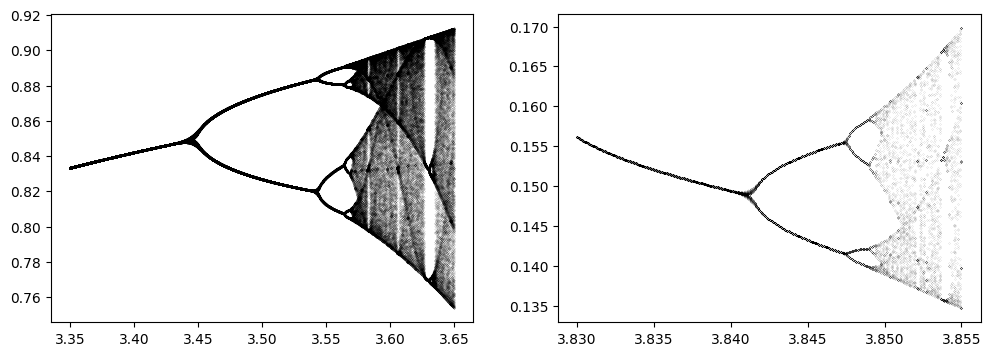
\includegraphics[scale=0.4]{images/period-doubling-and-zoom2.png}
\caption{Ampliação das regiões marcadas na figura anterior.}
\end{figure}

\end{columns}
\end{frame}
